\documentclass[compress]{beamer}

\usetheme{Hamburg}

\usepackage[T1]{fontenc}
\usepackage[utf8]{inputenc}

\usepackage{lmodern}

%\usepackage[english]{babel}
\usepackage[ngerman]{babel}

\usepackage{eurosym}
\usepackage{listings}
\usepackage{microtype}
\usepackage{units}
\usepackage{minted}

\lstset{
	basicstyle=\ttfamily\footnotesize,
	frame=single,
	numbers=left,
	language=C,
	breaklines=true,
	breakatwhitespace=true,
	postbreak=\hbox{$\hookrightarrow$ },
	showstringspaces=false,
	tabsize=4,
	captionpos=b,
	morekeywords={gboolean,gpointer,gconstpointer,gchar,guchar,gint,guint,gshort,gushort,glong,gulong,gint8,guint8,gint16,guint16,gint32,guint32,gint64,guint64,gfloat,gdouble,gsize,gssize,goffset,gintptr,guintptr,int8_t,uint8_t,int16_t,uint16_t,int32_t,uint32_t,int64_t,uint64_t,size_t,ssize_t,off_t,intptr_t,uintptr_t,mode_t}
}

\title{Vectorization}
\author{Oliver Heidmann}
\institute{Arbeitsbereich Wissenschaftliches Rechnen\\Fachbereich Informatik\\Fakultät für Mathematik, Informatik und Naturwissenschaften\\Universität Hamburg}
\date{2016-12-22}

\titlegraphic{
\includegraphics[width=0.75\textwidth]{logo}}

\begin{document}

\begin{frame}
	\titlepage
\end{frame}

\begin{frame}
	\frametitle{Gliederung (Agenda)}

	\tableofcontents[hidesubsections]
\end{frame}

\section{The problem at hand}
\subsection{Making code run faster}
\begin{frame}
    The Program: \newline
        Simulation/Game/Analytics which processes huge amounts of data.\newline
        It is already written in an data oriented style.        \newline \newline
    The Problem: \newline
        The execution time is way too high. \newline

    What can we do?
\end{frame}
\begin{frame}
    Steps of making code faster:
            \begin{itemize}
                \setlength\itemsep{0.25em}
                \item manual optimizations
                \item parallelization
                \item buying better hardware
                \item buying more hardware
            \end{itemize}

\end{frame}
\begin{frame}

    Steps of making code faster:
            \begin{itemize}
                \setlength\itemsep{0.25em}
                \item manual optimizations
                \item parallelization
                \setlength\itemsep{1em}
                
                \item => vectorization <=
                \item buying better hardware
                \setlength\itemsep{0.25em}
                \item buying more hardware
            \end{itemize}

\end{frame}
\section{What is vectorization?}
\subsection{Vector Units}
%=====================================

\begin{frame}[fragile]
    \frametitle{Vectorization}

What is Vectorization?\newline\newline
Vectorization allows us to compute multiple operations at once.\newline\newline
How is that possible?
    \begin{itemize}
        \item extended set of CPU instructions
    \end{itemize}
\end{frame}
%=====================================
\begin{frame}
    Important differences between instruction sets:
    \begin{itemize}
        \item SSE(Streaming SIMD Extensions)
            \begin{itemize}
                \item only single precision floats
                \item 8 128-bit vector registers
                \item first supported by intel pentium 3
            \end{itemize}
               \end{itemize}
   \end{frame}
   \begin{frame}
    Important differences between instruction sets:
    \begin{itemize}
        \item SSE(Streaming SIMD Extensions)
            \begin{itemize}
                \item only single precision floats
                \item 8 128-bit vector registers
                \item first supported int intel pentium 3
            \end{itemize}
        \item SSE2
            \begin{itemize}
                \item added support for 16-bit short, 32-int, 64-double-precision and 64-int
                \item added 8 new vector registers for x64
            \end{itemize}
               \end{itemize}
   \end{frame}

\begin{frame}
    Important differences between instruction sets:
    \begin{itemize}
        \item SSE(Streaming SIMD Extensions)
            \begin{itemize}
                \item only single precision floats
                \item 8 128-bit vector registers
                \item first supported int intel pentium 3
            \end{itemize}
        \item SSE2
            \begin{itemize}
                \item added support for 16-bit short, 32-int, 64-double-precision and 64-int
                \item added 8 new vector registers for x64
            \end{itemize}
        \item AVX/AVX2(Advanced Vector Extensions)
            \begin{itemize}
                \item now 256-bit registers
                \item added three-operand SIMDs
                \item added gather support
            \end{itemize}
        \end{itemize}
   \end{frame}

%=====================================

\begin{frame}[fragile]
    \frametitle{Vectorization}

What is Vectorization?\newline\newline
Vectorization allows us to compute multiple operations at once.\newline\newline
How is that possible?
    \begin{itemize}
        \item extended set of CPU instructions
        \item vector units
    \end{itemize}
\end{frame}
%=====================================
\subsection{Vector Units}
        \begin{frame}
        \frametitle{What are those units?}
        \begin{itemize}
            \item special computation units
                \item every modern CPU implements them
                \item calculate multiple results from multiple inputs in one instruction \newline 
                    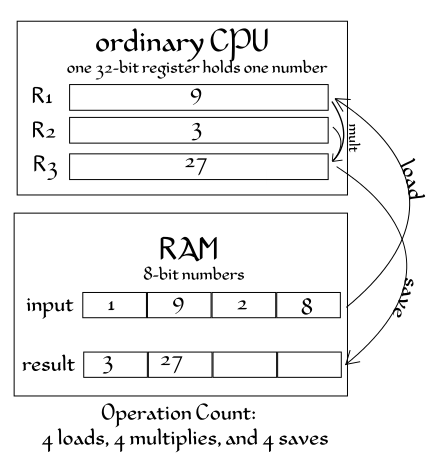
\includegraphics[width=0.38\textwidth]{Non-SIMD_cpu_diagram.png}     
                    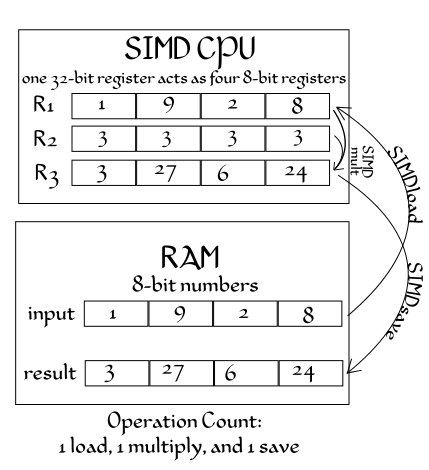
\includegraphics[width=0.38\textwidth]{SIMD_cpu_diagram.png}
        \end{itemize}

\end{frame}
\subsection{Vector Registers}
\begin{frame}[fragile]
    \frametitle{Vectorization}
What is Vectorization?\newline\newline
Vectorization allows us to compute multiple operations at once.\newline\newline
How is that possible?
    \begin{itemize}
        \item extended set of CPU instructions
        \item vector units
        \item vector registers 
    \end{itemize}
\end{frame}
\begin{frame}
    \frametitle{Vector Registers}
    \begin{itemize}
        \item extra registers on the CPU
        \item can store and load multiple values at once
    \end{itemize}
    \includegraphics[width=1\textwidth]{RegistersSizes.png}
\end{frame}
%=====================================
\begin{frame}
    \includegraphics[width=0.8\textwidth]{VectorRegisters.png}
\end{frame}

\subsection{Extended CPU vector instructions}
\begin{frame}[fragile]
    \frametitle{Vectorization}

What is Vectorization?\newline\newline
Vectorization allows us to compute multiple operations at once.\newline\newline
How is that possible?
    \begin{itemize}
        \item extended set of CPU instructions
        \item vector units
        \item vector registers 
    \end{itemize}
\end{frame}
%=====================================


\subsection{All in all}
\begin{frame}[fragile]
    \frametitle{Vectorization}
What is Vectorization?\newline\newline
Vectorization allows us to compute multiple operations at once.\newline\newline
How is that possible?
    \begin{itemize}
        \item extended set of CPU instructions
        \item vector units
        \item vector registers 
        \item everything implemented in silicon
    \end{itemize}
\end{frame}
%=====================================
\begin{frame}[fragile]
    \frametitle{Vectorization}
What is Vectorization?\newline\newline
Vectorization allows us to compute multiple operations at once.\newline\newline
How is that possible?
    \begin{itemize}
        \item vector units
        \item vector registers 
        \item extended set of CPU instructions
        \item everything implemented in silicon
    \end{itemize}
\end{frame}
%=====================================
\begin{frame}
    \frametitle{What speedup can we expect?}
    \begin{tabular}{c | c | c}
        type-width & 128-bit & 256-bit \\
        \hline
        8            & 1600\% &  3200\% \\
        16           & 800\% &   1600\% \\
        32           & 400\%  &   800\% \\
        64          & 200\% & 400\% \\ 
        \hline
    \end{tabular} 
    \newline
    \newline
    Real speedup will not be as huge
    \begin{itemize}
        \item overhead from loops
        \item cache misses/ memory access times
        \item data layout not perfect
    \end{itemize}
\end{frame}

%=====================================
\begin{frame}[fragile]
    \frametitle{Vectorization}
What is Vectorization?\newline\newline
Vectorization allows us to compute multiple operations at once.\newline\newline
How is that possible?
    \begin{itemize}
        \item vector units
        \item vector registers 
        \item extended set of CPU instructions
        \item everything implemented in silicon
    \end{itemize}
The effect:
    \begin{itemize}
        \item huge speedups
    \end{itemize}
\end{frame}
%=====================================
\section{Vectorizing code}
\subsection{Gcc Usage}
\begin{frame}
    \frametitle{How can I use vectorization?}
    The compiler does that for us if we tell him to.\newline
    Example for gcc:
    \begin{itemize}
        \item gcc standard optimizations do not vectorize 
        \item -O3 enables auto vectorization
        \item -O3 does it by using the -ftree-vectorize flag 
        \item -fopt-info-vec enables vectorization report
        \item -save-temps saves the temporary files eg. assembler code
    \end{itemize}
\end{frame}
\subsection{Code requirements}
\begin{frame}[fragile]
    \frametitle{What makes my code eligible for vectorization?}
    \begin{itemize}
        \item calculations over arrays
        \item code must be in the innermost loop 
        \item no if statements
        \item only inlined functions 
        \item continuous data chunks
    \end{itemize}
\end{frame}
\subsection{data organisation}
\begin{frame}[fragile]
    \frametitle{data organisation}
    Context: distance calculations; sqrt(x * x + y * y + z * z)
    \begin{minted}{c++}
        struct vector               struct particle
        {                           {
            float x;                    vector pos;
            float y;                    vector velo;
            float z;                    vector accel;
        }                           }
        
    \end{minted}
    This wont work well
    \begin{itemize}
        \item data is not coherent
    \end{itemize}
\end{frame}
  \begin{frame}[fragile]
    \frametitle{data organisation}
    Context: distance calculations; sqrt(x * x + y * y + z * z)
    \begin{minted}{c++}
        struct vectors              struct particles
        {                           {
            float x[particle_cnt];    vectors pos;
            float y[particle_cnt];    vectors velo;
            float z[particle_cnt];    vectors accel;
        }                           }
        
    \end{minted}
    This will work well
    \begin{itemize}
        \item data is now coherent
    \end{itemize}
\end{frame}    
\begin{frame}
    \includegraphics[width=1\textwidth]{datalayout_results.png}
\end{frame} 
\subsection{Example Vectorization}
\begin{frame}[fragile]
    \begin{minted}{c++}
void test(float * vec1, float * vec2, float * res) {
    for (unsigned long i = 0; i < vector_size; i++) {
        res[i] += vec2[i] * vec1[i];
    }
}
    \end{minted}
\end{frame}
\begin{frame}
       \begin{itemize}
        \item program checks for overlapping arrays parts
        \item program needs to check for aliasing            
    \end{itemize}
 \begin{tabbing}
    The restrict keyword: \\
    ~~~~ \= Tells the compiler that the pointers are not aliased. \\
    \> Meaning that the (sub)arrays are not overlapping or the same.
\end{tabbing}

\end{frame}

\begin{frame}[fragile]
    \begin{minted}{c++}
void test(float *__restrict vec1,
          float *__restrict vec2,
          float *__restrict res) {
    for (unsigned long i = 0; i < vector_size; i++) {
        res[i] += vec2[i] * vec1[i];
    }
}
    \end{minted}
\end{frame}
\begin{frame}
    \begin{itemize}
        \item needs information about type boundaries
    \end{itemize}
 \begin{tabbing}
     \_\_attribute\_\_((\_\_aligned\_\_(type\_size))) :\\
~~~~\= Tells the compiler the size of the type in bit. \\
\> So that it is known how big a to be loaded bit word is.\\
\> Otherwise size will be checked at runtime.
\end{tabbing}
\end{frame}
\begin{frame}[fragile]
    \begin{minted}[fontsize=\footnotesize]{c++}
constexpr size_t float_size = sizeof(float) * 8;
typedef float float_32 __attribute__((__aligned__(float_size)))

void test(float_32 *__restrict vec1,
          float_32 *__restrict vec2,
          float_32 *__restrict res) 
{
    for (unsigned long i = 0; i < vector_size; i++) {
        res[i] += vec2[i] * vec1[i];
    }
}
\end{minted}
\end{frame}


\section{Conclusion}
\subsection{Pro/Cons}
\begin{frame}
    \frametitle{Vectorization: Pros/Cons}
    Pros:
    \begin{itemize}
        \item depending on numeric type we can gain huge to immense speedup
        \item most modern systems support vectorization
        \item no extra cost for new hardware
        \item no extra software needed
    \end{itemize}
    Cons:
    \begin{itemize}
        \item complicated to implement for object oriented design
        \item exact result only visible in assembler code 
    \end{itemize}
\end{frame}

\subsection{Conclusion}
\begin{frame}
	\frametitle{Conclusion}

	\begin{itemize}
        \item vectorization is a from of optimization
            \begin{itemize}
                \item supported by modern compilers (gcc 4.6 and onward)
			\item supported in modern hardware
            \item when done right gives immense speedup
		\end{itemize}
		\item Vectorizing
		\begin{itemize}
			\item compiler does it for us
			\item if it gets enough info
            \item needs coherent data layout 
		\end{itemize}
        %\item Quelle: \cite{Quelle2012}
	\end{itemize}
\end{frame}
\section{further material}
\begin{frame}
    \begin{itemize} 
                \setlength\itemsep{1em}
        \item talk about vectorization by Ulrich Drepper \newline
            \url{https://www.youtube.com/watch?v=DXPfE2jGqg0}
        \item talk about vectorization by James Reinders \newline
            \url{https://www.youtube.com/watch?v=hyZMssi_gZY&t=1640s}
        \item Article about auto vectorization (caution!  for gcc 4.7) \newline
            \url{https://locklessinc.com/articles/vectorize/}
    \end{itemize}

\end{frame}

\section{Literatur}
\subsection*{}

\begin{frame}
	\frametitle{Literatur}

	\bibliographystyle{alpha}
	\bibliography{literatur}
\end{frame}

\end{document}
